\documentclass[tikz, border=2pt]{standalone}

\usepackage{amsmath,amssymb}
\usepackage{pgfplots}
\pgfplotsset{compat=1.18}
\usepackage{xcolor}

\definecolor{utnblue}{RGB}{0, 51, 102}
\definecolor{utnred}{RGB}{204, 0, 0}

\begin{document}
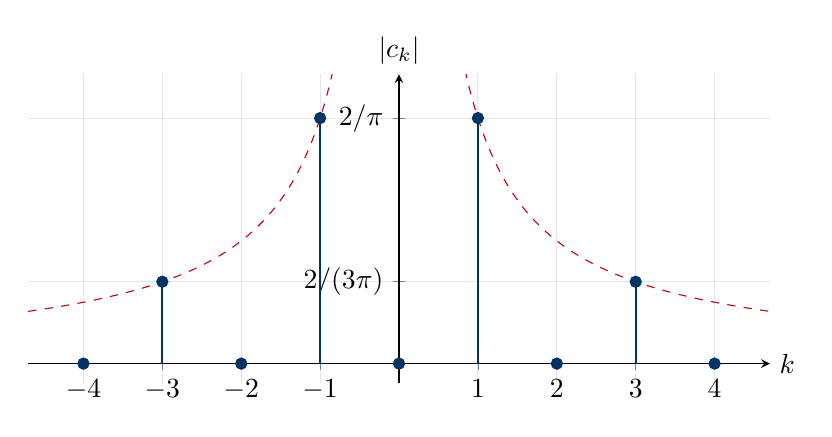
\begin{tikzpicture}

\begin{axis}[
    width=11cm, height=5.5cm,
    xmin=-4.7, xmax=4.7,
    ymin=-0.05, ymax=0.75,
    xtick={-4,-3,-2,-1,0,1,2,3,4},
    ytick={0, 0.2122, 0.6366},
    yticklabels={$0$, $2/(3\pi)$, $2/\pi$},
    xlabel={$k$},
    ylabel={$|c_k|$},
    axis lines=middle,
    enlargelimits=false,
    grid=major,
    grid style={gray!20},
    every axis x label/.style={at={(ticklabel* cs:1)}, anchor=west},
    every axis y label/.style={at={(ticklabel* cs:1)}, anchor=south},
]
% Envolvente 2/(|k| pi) sobre k impar
\addplot[utnred, dashed, samples=300, domain=0.5:4.7]
    ({x}, {2/(x*pi)});
\addplot[utnred, dashed, samples=300, domain=-4.7:-0.5]
    ({x}, {-2/(x*pi)});
% Stems
\addplot+[utnblue, thick, ycomb, mark=*, mark options={fill=utnblue, scale=0.9}]
    coordinates {
        (-4, 0) (-3, 0.2122) (-2, 0) (-1, 0.6366) (0, 0)
        (1, 0.6366) (2, 0) (3, 0.2122) (4, 0)
    };
\end{axis}

\end{tikzpicture}
\end{document}
